\documentclass[12pt]{article}
\usepackage{geometry}
\geometry{a4paper}
\usepackage{fancyhdr}
\usepackage{graphicx}
\usepackage[official]{eurosym}
\usepackage{wallpaper}
\usepackage{tabularx}
\usepackage{Sweave}
\begin{document}

\pagestyle{fancy}
\input{ctbtitle.tex}
\cfoot{\footnotesize confidential}
\rfoot{\footnotesize \thepage}
\section{Final arm's length ranges and their application}
\subsection{General provisions}
Anvis Group's transfer pricing system for intra-group services and contract R\&D relies on the transactional net margin method. At budget, the arm's length transfer price for these services is determined using a profit mark-up consistent with the mid-point of the respective interquartile range. The actual result is regularly reviewed (at least after 6 months). A transfer pricing adjustment is made whenever the respective service entity's actual profit is not within the corresponding arm's length range. The adjustment is made to the range's upper or lower bound whatever is closest to the actual result achieved.\\[0.2cm]
The adjustment is a retro-active adjustment ensuring that the actual results are within the arm's length range. This is largely consistent with Anvis Group's current practice. In order to charge each recipient with the actual cost incurred on its behalf/the actual benefits received, Anvis Deutschland GmbH (AVS002) issues already debit or credit notes.\\[0.2cm]
As outlined below, the arm's length ranges reflect period averages. Accordingly, a transfer pricing adjustment back to the closest upper or lower bound can be based on period averages as well. In order to limit the transfer pricing related worklaod the comparison will be based on the respective Anvis entities' annual data.\\[0.2cm]
The arm's length ranges are to be reviewed regularly.\begin{itemize}
  \item just adding new data (effectively employ a moving average approach)
  \item conduct a completely new comparables search
  \item recalculate the necessary comparability adjustments
\end{itemize}
Bureau van Dijk's \emph{tp catalyst} primarily provides convenient access to a comprehensive database (Amadeus) of European companies. The data available cover: \begin{itemize}
  \item trade and business descriptions
  \item industry classifications (e.g. NACE, ...)
  \item financial data presented in a global standard format and a common currency (e.g. K\euro) for several years
  \item ownership information including and a corresponding independence index
  \item management / directors
\end{itemize}
\begin{figure}[!hbtp]
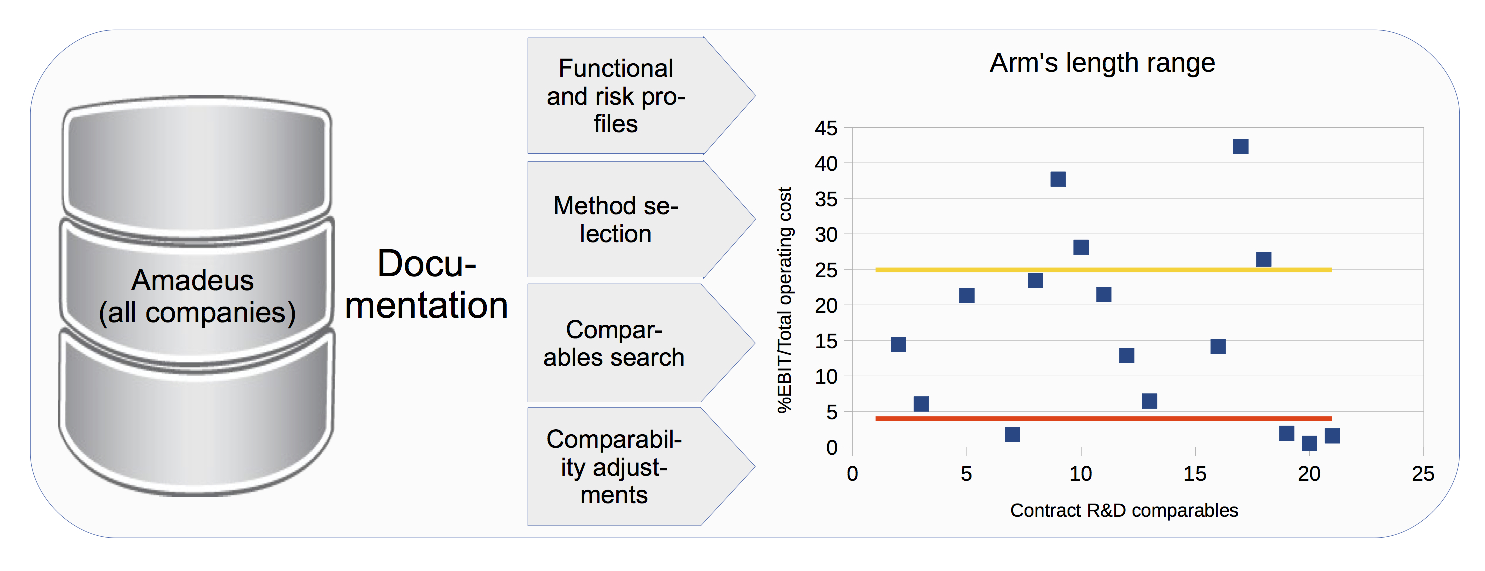
\includegraphics[width=1.0\textwidth]{./tpCatalyst.eps}
\caption{\footnotesize Bureau van Dijk's \emph{tp catalyst}'s major features}
\label{tpCatalyst}
\end{figure}
In addition to providing access to company data, \emph{tp catalyst} effectively supports the transfer pricing related outside evidence work (Figure \ref{tpCatalyst}). It allows to define the tested party's functional and risk profile. The corresponding segmented financial data can be keyed in and made avaialble for further analysis - in particular for determining comparability adjustments as and when required. With respect to comparables search \emph{tp catalyst} provides a full audit trail from the universe of potential comparables to the finally accepted set of functionally comparable companies used to determing the selected profit level indicator's arm's length range.
\section{Industry code based and keyword based searches define the universe of potential comparables}
The search criteria are derived from Anvis Group's service companies' functional and risk profile.
\begin{table}[!hbtp]
\begin{tabularx}{1.0\textwidth}{|l|X|X|c}
\hline \textbf{Major Service Activity} &  \textbf{Functions performed} & \textbf {Risks assumed}\\
\hline
\small Contract R\&D & \small The product engineering ranges from\begin{itemize} \item \small product specification \item \small product development \item \small production of samples \end{itemize} & \small The risk exposure is limited as the plants cover the cost (including possible budget overruns)\\
\hline
\end{tabularx}
\caption{\footnotesize Anvis Service companies - functional and risk profile}
\label{FunProf}
\end{table}


\section{The contract service comparables}
\section{The contract R\&D comparables}
\subsection{The universe of potential contract R\&D comparables }
The transfer pricing keyword based search identified 211 potential contract R\&D comparables (see Table \ref{UCRaD_02}).These 211 potential comparables stem from a base population of more than 3 Mio. active European companies with 3 consecutive years of financial data (covering the 3 year period 2011 - 2013).The transfer pricing specific keywords used were:\begin{itemize}
  \item testing and analysis
  \item laboratory, research, and r\&d.
\end{itemize} Bureau von Dijk's \emph{tp catalyst} offers a set of standardized transfer pricing related keywords which cover a wide range of functions to be considered when determining an affiliated entity's functanal and risk profile. Obviously, these keywords are not a full representation of the comprehensive R\&D functions Anvis Group's service companies provide. Activities such as product engineering and/or product development are not explicitly taken into account. 
\begin{table}[!hbtp]
\centering
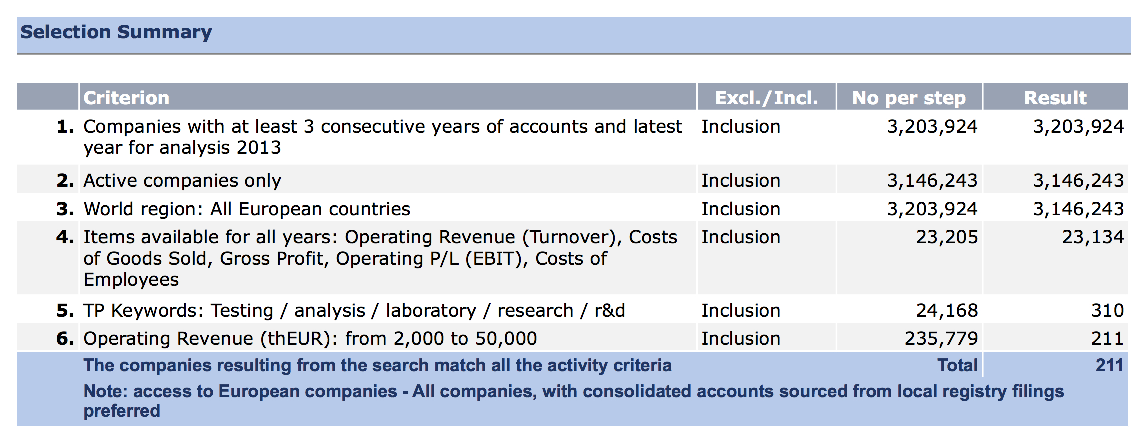
\includegraphics[width=1.0\textwidth]{./UCRaD_02.eps}
\caption{\footnotesize Universe of potential contract R\&D comparables employing transfer pricing keywords}
\label{UCRaD_02}
\end{table}
According to Figure \ref{UCRaD_02} most of the companies within the universe of potential comparables do not qualify as potential comparable due to the lack of meaningful financial data throughout a minimum base period of 3 years. The additional size criterion, which requires the potential comparable contract R\&D companies to report annual sales between \euro 2 Mio and  \euro 50 Mio eliminates fewer companies from further review.\\[0.2cm]
\begin{table}[!hbtp]
\centering
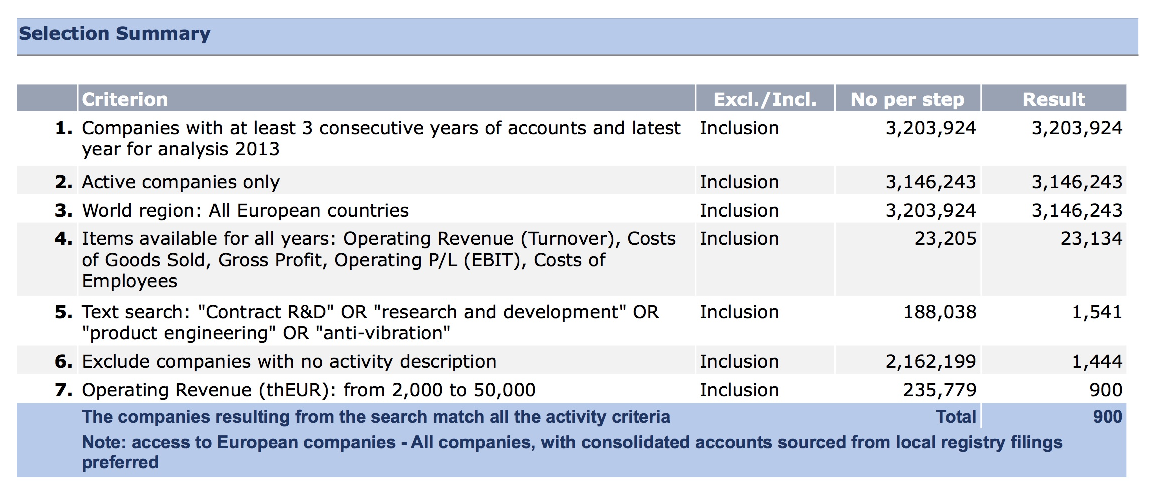
\includegraphics[width=1.0\textwidth]{./UCRaD_04.eps}
\caption{\footnotesize Universe of potential contract R\&D comparables employing general keywords}
\label{UCRaD_04}
\end{table}
In order to assess the sensitivity of the order of magnitude of the universe of potential comparables with respect to the search approach an alternative search has been conducted. The analysis takes into account the following keywords: \begin{itemize}
  \item contract R\&D, product development
  \item product engineering or anti-vibration
\end{itemize}
Table \ref{UCRaD_04} shows that a keyword search not limited to the specific transfer pricing keywords leads to a substantially larger universe of potential comparables of 900 firms. The additional selection criteria already discussed were not changed. The increase in the sizes of the universe is, therefore, attributable to the change in keywords only.\\[0.2cm]
With the various industry codes (e.g. Statistical classification of economic activities in the European Communities - NACE) \emph{tp catalyst} offers another way for defining the universe of potential contract R\&D comparables.
\begin{table}[!hbtp]
\centering
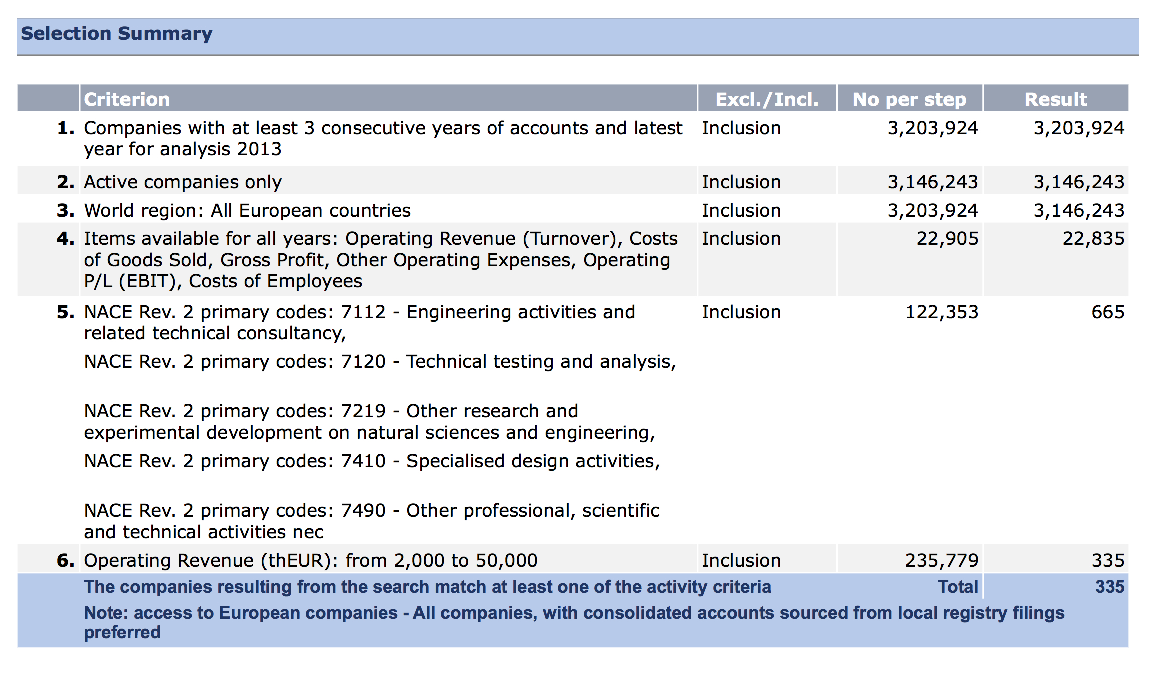
\includegraphics[width=1.0\textwidth]{./UCRaD_03a.eps}
\caption{\footnotesize Universe of potential contract R\&D comparables based on NACE codes}
\label{UCRaD_03b}
\end{table}

So far, the criteria used to arrive at the universe of potential comparables focus on functions, the relevant markets, and the the size of the operations. However,

\begin{figure}[!hbtp]
\includegraphics{AVS_OS_Docu-002}
\caption {Test}
\end{figure}
\section{Appendices}
This sections provides supplementary information to the data sets used. The company information available was primarily retrieved from Bureau van Dijks \emph{tp catalyst}. The Anvis license is limited to European companies included in the Amadeus all companies data base Bureau van Dijk maintains.\\[0.2cm]
In order to faciliate a more detailed analysis, the results from the different searches were retrieved and uploaded in an R \cite{Team:2014aa} database. \emph{tp catalyst} provides detailed Excel output and R is able to read .csv data. The required .csv input files were, therefore, constructed from the respective Excel results.
\subsection{Data used and integrity check}
The retrieved financial and general data are stored in several R objects for further analysis (see Table \ref{RObjCRaD} for contract R\&D). 
\begin{table}[!hbtp]
\begin{tabularx}{1.0\textwidth}{|l|X|X|X|X|c}
\hline R Object & Description & Years & Remarks\\
\hline
\small ContRaD\_01 & \small Initial set of financials (not fully retrieved) 2 & \small 5 & \small Not used for policy purposes\\
\small ContRaD\_01b & \small Revised initial sample. Search was adjusted to select contract R\&D companies reporting salaries and wages.& 5 & \small Not used for policy purposes\\
\small ContRaD\_02 & \small Universe of potential comparables defined using special transfer pricing search keywords only & \small 3 (2011 - 2013) & \small Part of the final contract R\&D universe.\\
\small ContRaD\_02b & \small Search criteria similar to ContRaD\_02, however limited to a 5 year period. & \small 5 (2009 - 2013) & \small Created to assess the reference period's impact on the universe.\\
\small ContRaD\_03a & \small Universe of potential comparables based on NACE codes. & \small 3 (2011 - 2013) & \small Part of the final contract R\&D universe\\
\small ContRaD\_03b & \small Search criteria similar to ContRaD\_03a, however limited to a 5 year period. & \small 5 (2009 - 2013) & \small Created to assess the reference periods's impact ont the universe.\\
\small ContRaD\_04 & \small Universe of potential comparables defined using general search keywords. & \small 3 (2011 - 2013) & \small Part of the final contract R\&D universe.\\
\small ContRaD\_04b & \small Search criteria similar to ContRaD\_04, however limited to a 5 year period. & \small 5 (2009 - 2013) & \small Created to assess the reference period's impact on the universe.\\
\hline
\end{tabularx}
\caption{\footnotesize R data objects available for contract R\&D analysis}
\label{RObjCRaD}
\end{table}
\begin{table}[!hbtp]
\begin{tabularx}{1.0\textwidth}{|l|X|X|X|X|c}
\hline R Object & Description & Years & Remarks\\
\hline
\small ContServ\_01\\
\small ContServ\_02\\
\small ContServ\_03\\
\hline
\end{tabularx}
\caption{\footnotesize R data objects available for contract services analysis}
\label{RObjCServ}
\end{table}
\subsection{References}
\bibliography{LaTexLiterature}
\bibliographystyle{abbrv}
\end{document}
